\section{Global Scoring Functions}

\label{sec4p5}

First, we adapt from the BaB-SR \cite{BaB} and FSB \cite{FSB} functions (replacing the symbols from the original paper with those used in our paper.), selecting a node to branch on for BaB, {\em  global scoring} (GS) functions to select nodes for pMILP. Intuitively, we extract the scoring $s_{SR}$ and $s_{FSB}$ from both BaB-SR and FSB, as the BaB bounding step is not adapted for pMILP. They both work by backpropagating gradients vectors $\bm{\lambda}$ from the neurons under consideration in layer $n$, back to neurons to be potentially selected. To do so, they consider the rate of $\ReLU(\bm{u}_k)$ to be 
$r(\bm{u}_k)=\frac{\max(0,\UB(\bm{u}_k))}{\max(0,\UB(\bm{u}_k))-\min(0,\LB(\bm{u}_k))} \in [0,1]$, 
with $r(b)=0$ iff $\UB(b)\leq 0$ and $r(b)=1$ iff $\LB(b)\geq 0$.

\begin{align*}
\bm{\lambda}_{n-1} = -{(\bm{W}^n)}^T\bm{1}, \hspace*{4ex}  	\bm{\lambda}_{k-1} = {(\bm{W}^k)}^T\big( r(\bm{u}_k) \odot\bm{\lambda}_{k}\big) \hspace*{4ex}  k\in [n-1,2]
\end{align*}


Then, the scoring functions $\bm{s}_{SR}$ and $\bm{s}_{FSB}$ for ReLUs in layer $k$ are computed by approximating how each node would impact the neurons in layer $n$, by also factoring in the bias $\bm{b}_k$ in different ways:

\begin{align*}
	\bm{s}_{SR}(k) =& %\bm{1}_{\bm{u}_k>0,\bm{l}_k<0} \odot
	\Biggl\lvert r(\bm{u}_k) \odot \LB(\bm{u}_k) \odot \max(\bm{\lambda}_{k},0)
	+ \max\{0,\bm{\lambda}_{k}\odot\bm{b}_{k}\}-r(\bm{u}_k) \odot\bm{\lambda}_{k}\odot\bm{{b}}_{k}
	\Biggr\rvert  \\
	\bm{s}_{FSB}(k) =& \Biggl\lvert r(\bm{u}_k) \odot \LB(\bm{u}_k) \odot \max(\bm{\lambda}_{k},0)
	+ \min\{0,\bm{\lambda}_{k}\odot\bm{b}_{k}\}-r(\bm{u}_k) \odot\bm{\lambda}_{k}\odot\bm{{b}}_{k}
	\Biggr\rvert
\end{align*}

In case where the bias is 0, then there is no difference between $s_{SR}$ and $s_{FSB}$.
Then, unstable ReLU (with $\LB(u_k) < 0 < \UB(u_k)$) are ranked using these scores, to select the most important ReLUs, as stable ReLUs are linear, thus they are already treated correctly.


\begin{figure}[t!]
	\centering
	\begin{tikzpicture}
		
		\node[circle, draw= black, thick, minimum width = 20,
		minimum height = 20] (input1) {$n$};
		
		\node[circle, draw= black, thick, minimum width = 20,
		minimum height = 20] (input2) at ($(input1) + (0,-1.5)$) {$n'$};
		
		
		% Hidden layers
		
		\node (hidden10) at ($(input1) + (2.5,0.6)$) {$[-1,1]$};
		
		\node (hidden20) at ($(input1) + (2.5,-1.5-0.6)$) {$[-10,11]$};
		
		\node (hidden50) at ($(input1) + (7.5,0.6)$) {$[-1,1]$};
		
		\node (hidden60) at ($(input1) + (7.5,-1.5-0.6)$) {$[0,0.5]$};
		
		
		\node[circle, draw= black, thick, minimum width = 20,
		minimum height = 20] (hidden1) at ($(input1) + (2.5,0)$) {$a$};
		\node[circle, draw= black, thick] (hidden2) at ($(input1) + (2.5,-1.5)$) {$a'$};
		
		\node[circle, draw= black, thick, minimum width = 20,
		minimum height = 20] (hidden3) at ($(input1) + (5,0)$){$\hat{a}$};
		\node[circle, draw= black, thick] (hidden4) at ($(input1) + (5,-1.5)$) {$\hat{a}'$};
		
		
		\node[circle, draw= black, thick, minimum width = 20,
		minimum height = 20] (hidden5) at ($(input1) + (7.5,0)$){$b$};
		\node[circle, draw= black, thick] (hidden6) at ($(input1) + (7.5,-1.5)$) {$b'$};
		
		
		
		
		% Output layer
		\node[circle, draw= black, thick, minimum width = 20,
		minimum height = 20] (output1) at ($(input1) + (10,0)$){$\hat{b}$};
		
		\node[circle, draw= black, thick, minimum width = 20,
		minimum height = 20] (output2) at ($(input1) + (10,-1.5)$){$\hat{b}'$};
		
			\node[circle, draw= black, thick, minimum width = 20,
		minimum height = 20] (output3) at ($(input1) + (12.5,0)$){$z$};
		
		
		% Connections
		
		\draw[->,thick] ($(input1) + (-1.5,0)$) -- (input1) node[midway, above] {$[-1,1]$};
		
		\draw[->,thick] ($(input1) + (-1.5,-1.5)$) -- (input2) node[midway, above] {$[-1,1]$};
		
		\draw[->,thick] (input1) -- (hidden1) node[near start, above] {$1$};
		\draw[->,thick] (input1) -- (hidden2)node[near start, below] {$-10$};
		
		\draw[->, thick] (input2) -- (hidden2)node[near start, below] {$0.5$};
		
		
		
		
		
		\draw[->, thick] (hidden1) -- (hidden3);
		\draw[->, thick] (hidden2) -- (hidden4);
		
		
		
		
		
		\draw[->, thick] (hidden3) -- (hidden5) node[near start, above] {{\color{red}$c$}};			
	
		\draw[->,thick] (hidden4) -- (hidden5)node[near start, above] {$1$};
		\draw[->,thick] (hidden4) -- (hidden6)node[near start, below] {$1$};
		
		
		\draw[->,thick] (hidden5) -- (output1);
		\draw[->,thick] (hidden6) -- (output2);
		
		\draw[->,thick] (output1) -- (output3)node[near start, above] {{\color{red}$d$}};
		\draw[->,thick] (output2) -- (output3)node[near start, below] {$1$};
		
		
	\end{tikzpicture}
	\caption{A simple example with parametric weights {\color{red}$c$} and {\color{red}$d$}}
	\label{img:FSB_example}
\end{figure}




Consider the example in Fig. \ref{img:FSB_example}. It has no bias so $s_{SR}=s_{FSB}$.
We have $\lambda(b)=d$, $\lambda(a)=\frac{cd}{2}$.
Let us do a case analysis:
The most favorable cases are $c < 0 < d$ and $d < 0 < c$: 
as $cd <0$, we have $s_{FSB}(a)=\max(0,\frac{cd}{4}) = 0$.
Now, $a$ and $\hat{a}$ need to be minimized in order to maximize $z$, because $cd <0$. 
For the triangle approximation (see Fig. \ref{triangle}), having a value $sol(a)$ for $a$, the minimal value for $\hat{a}$ is $\ReLU(sol(a))$. If we open $a$, then the value for $\hat{a}$ will also be $\ReLU(sol(a))$. That is, opening this ReLU is not helping in the approximation of $z$, as correctly predicted by the score $s_{FSB}(a)= 0$.



Case $c>0,d>0$: $s_{FSB}(a)=\frac{cd}{4}$.
The value of $a,\hat{a},b,\hat{b}$ should be maximized to maximize the value of $z$, because $W_{bz}=d>0$ and $W_{ab}=c>0$. 
%Each variation of $b$ by $\Delta(b)$ will have an impact $r(b) \cdot \Delta(b)=\frac{\Delta(b)}{2}$ on the value of $\hat{b}$, and thus $\frac{d \Delta(b)}{2}$ on $z$. 
Now, let us call $sol(a)$ the maximum value for $a$.
The maximum value for $\hat{a}$ is $r(a)\cdot (sol(a)-LB(a))$ according to the triangle approximation when $\ReLU(a)$ is not opened. Now, if $\ReLU(a)$ is opened, then 
the value of $\hat{a}$ is $\ReLU(sol(a))$: the difference is at most $r(a) \cdot LB(a) = \frac{1}{2}$. The difference $\Delta(b)$ for the value of $b$ is thus at most $\frac{c}{2}$, which means a difference at most $\frac{c}{4}$ for $\hat{b}$, using the upper function of the triangle approximation of rate $r(b)$, as the value of $\hat{b}$ should be maximized.
This means a difference of at most $\frac{cd}{4}$ on the value of $z$, which is what is computed by $s_{FSB}(a)$. Of course, the difference of opening $\ReLU(a)$ could also be 0 e.g. if $\sol(a)=\LB(a)$ or $\sol(a)=\UB(a)$.

The last case is the most problematic: 
Case $c<0,d<0$, implying that $s_{FSB}(a)=\frac{cd}{4}$, because $cd >0$.
As for the case of $c>0, d>0$, opening $\ReLU(a)$ will have an impact on the value of $\hat{a}$,
at most $\frac{1}{2}$, and hence a change $\Delta(b)$ of at most $\frac{c}{2}$ on the value of $b$.
However, as $d<0$, value of $\hat{b}$ needs to be minimized. That is, the value of $\hat{b}$ will be the value of $\ReLU(sol(b))$, and the change in $\hat{b}$ will be either 0 in case $sol(b)<0$ (phase 0 of ReLU),
or $\Delta(b)<\frac{c}{2}$ otherwise (phase Id of ReLU), that is, $z$ will be modified by 
either 0 or $d \Delta(b)<\frac{cd}{2}$, as compared with $s_{FSB}(a)=\frac{cd}{4}$.



\begin{figure}[t!]
	\begin{tikzpicture}[scale=1, >=stealth]
		
		% Draw axes
		\draw[->] (-5,0) -- (4,0) node[right] {$a$};
		\draw[->] (0,-1) -- (0,3) node[above] {$\hat{a}$};
		
		% Draw ReLU function
		\draw[line width=0.4mm, blue] (-3,0) -- (0,0);
		\draw[thick, blue] (0,0) -- (2.5,2.5) node[below, shift={(-1.1,-1.9)}] {$\hat{a} = \ReLU(a)$};
		\draw[thick, blue] (-3,0) -- (2.5,2.5) node[above, shift={(-6.5,-2)}] {$\hat{a} = \frac{\UB}{\UB-\LB} (a-\LB)$};
		
		% Add labels
		\draw[dashed] (2.5,0) -- (2.5,2.5) -- (0,2.5); % Optional grid
		\node[below left] at (0,0) {$0$};
		
		% Add tick marks
		
		\foreach \x in {2.5}
		\draw[shift={(\x,0)}] (0,0.1) -- (0,-0.1) node[below] {$\UB$};
		\foreach \x in {-3}
		\draw[shift={(\x,0)}] (0,0.1) -- (0,-0.1) node[below] {$\LB$};
	
		\foreach \y in {2.5}
		\draw[shift={(0,\y)}] (0.1,0) -- (-0.1,0) node[left] {$\UB$};
		
		
	\end{tikzpicture}
		\caption{Triangle approximation}
	\label{triangle}
	\end{figure}



\begin{figure}[t!]
	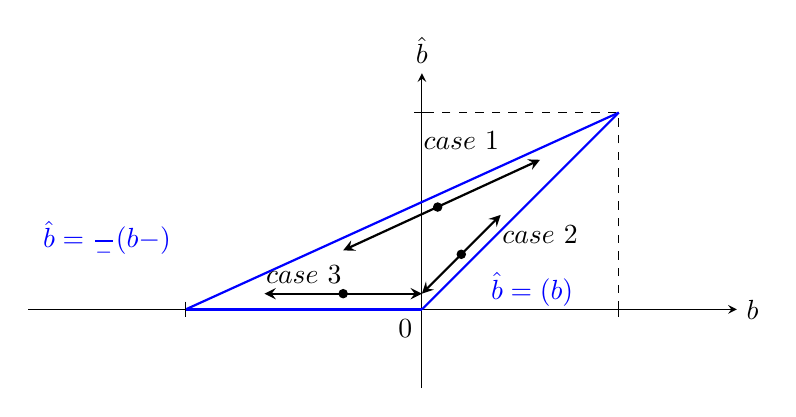
\begin{tikzpicture}[scale=1, >=stealth]
		
		% Draw axes
		\draw[->] (-5,0) -- (4,0) node[right] {$b$};
		\draw[->] (0,-1) -- (0,3) node[above] {$\hat{b}$};
		
		% Draw ReLU function
		\draw[line width=0.4mm, blue] (-3,0) -- (0,0);
		\draw[thick, blue] (0,0) -- (2.5,2.5) node[below, shift={(-1.1,-1.9)}] {$\hat{b} = \ReLU(b)$};
		\draw[thick, blue] (-3,0) -- (2.5,2.5) node[above, shift={(-6.5,-2)}] {$\hat{b} = \frac{\UB}{\UB-\LB} (b-\LB)$};
		
		% Add labels
		\draw[dashed] (2.5,0) -- (2.5,2.5) -- (0,2.5); % Optional grid
		\node[below left] at (0,0) {$0$};
		
		% Add tick marks
		
		\foreach \x in {2.5}
		\draw[shift={(\x,0)}] (0,0.1) -- (0,-0.1) node[below] {$\UB$};
		\foreach \x in {-3}
		\draw[shift={(\x,0)}] (0,0.1) -- (0,-0.1) node[below] {$\LB$};
		
		\foreach \y in {2.5}
		\draw[shift={(0,\y)}] (0.1,0) -- (-0.1,0) node[left] {$\UB$};
		
		\draw[<->, thick] (0, 0.2) -- (1, 1.2) node[above,shift={(0.5,-0.5)}] {$case\ 2$};
		\filldraw[black] (0.5, 0.7) circle (1.5pt);
		
		\draw[<->, thick] (0, 0.2) -- (-2, 0.2) node[above,shift={(0.5,0)}] {$case\ 3$};
		\filldraw[black] (-1, 0.2) circle (1.5pt);
		
		
		\draw[<->, thick] (-1, 0.75) -- (1.5, 1.9) node[above,shift={(-1,0)}] {$case\ 1$};
		\filldraw[black] (0.2, 1.3) circle (1.5pt);
		
	\end{tikzpicture}
	\caption{Different cases of node $b$}
	\label{node:b}
\end{figure}

We call {\em global scoring} (GS) such functions $s_{FSB},s_{SR}$  because they score ReLUs as accuratly as possible, considering that they do not have access to the solution $sol(a),sol(b)$ values. This analysis already hints at our novel ranking function, that will be solution-aware to be more accurate.
	



\iffalse
\begin{figure}[t!]
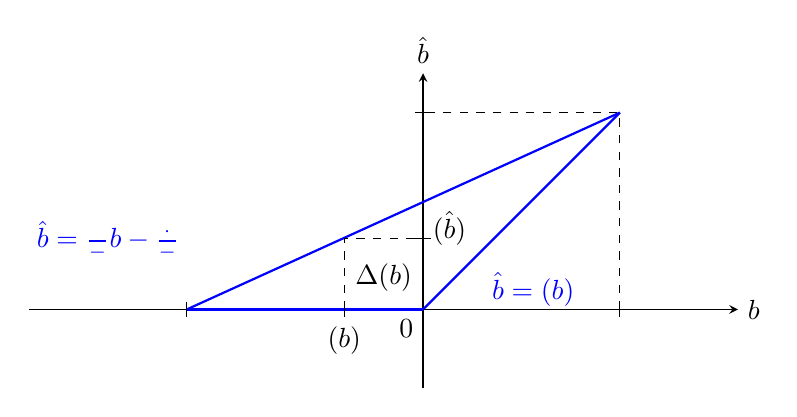
\begin{tikzpicture}[scale=1, >=stealth]
	
	% Draw axes
	\draw[->] (-5,0) -- (4,0) node[right] {$b$};
	\draw[->] (0,-1) -- (0,3) node[above] {$\hat{b}$};
	
	% Draw ReLU function
	\draw[line width=0.4mm, blue] (-3,0) -- (0,0);
	\draw[thick, blue] (0,0) -- (2.5,2.5) node[below, shift={(-1.1,-1.9)}] {$\hat{b} = \ReLU(b)$};
	\draw[thick, blue] (-3,0) -- (2.5,2.5) node[above, shift={(-6.5,-2)}] {$\hat{b} = \frac{\UB}{\UB-\LB} b-\frac{\UB\cdot\LB}{\UB-\LB}$};
	
	% Add labels
	\draw[dashed] (2.5,0) -- (2.5,2.5) -- (0,2.5); % Optional grid
	\node[below left] at (0,0) {$0$};
	
	% Add tick marks
	
	\foreach \x in {2.5}
	\draw[shift={(\x,0)}] (0,0.1) -- (0,-0.1) node[below] {$\UB$};
	\foreach \x in {-3}
	\draw[shift={(\x,0)}] (0,0.1) -- (0,-0.1) node[below] {$\LB$};

	\foreach \y in {2.5}
	\draw[shift={(0,\y)}] (0.1,0) -- (-0.1,0) node[left] {$\UB$};
	
	\draw (-1,0.1) -- (-1,-0.1) node[below] {$\sol(b)$};
	\draw[dashed] (-1,0) -- (-1,0.9) -- (0,0.9);
	\draw (-0.1,0.9) -- (0.1,0.9) node[right, shift={(-0.1,0.13)}] {$\sol(\hat{b})$};
	\node at (-0.5,0.4) {$\Delta(b)$};
	
\end{tikzpicture}
	\caption{}
\label{img:Utility}
\end{figure}
\fi


\iffalse
\subsection*{An example when FSB is not accurate}

See the figure \ref{img:FSB_example}. When the algorithm considers neurons in the layer of $a,a'$, FSB will think $a$ is important, but Utility will think it is not important (Utility value is 0).

Although this example is extreme, similar situations frequently occur in practice.

\subsection*{Comparison on MNIST}

Here we use the network named MNIST $5\times 100$ and a hard image to compare the effect of FSB and Utility function. 

We fix an intermediate bound data for layers before the third hidden layer, and use different methods based on this bound to compute the upper and lower bounds of neurons in the second and third hidden layer.

The plot shows that when only considering neurons in one layer before the target layer, we are significantly better.


\subsection*{Comparison on CIFAR10}

Here we use the network named CNN-B-adv and a hard image to compare the effect of FSB and Utility function. 

We fix an intermediate bound data for layers before the target layers, and use different methods based on this bound to compute the output layer.

The plot shows that our Utility function is significantly better than FSB, and other methods.
\fi
